
\section{Method}
In this section, we will describe the methods used for face and emotion recognition. We also discuss the datasets and propose the methods we will use to make use of them. We propose these methods considering that we need to achieve a minimum viable product for our robot. With this project, we aim to produce a physical prototype, so we have to consider that experimental results will impact the final implementation of the features and how much of a compromise between quality and performance we are willing to make. 



\subsection{FERPlus Dataset}

The FERPlus dataset, published by Barsoum et al. \cite{BarsoumICMI2016}, is an improvement over the previous FER\cite{FER2013} dataset published for a \emph{Kaggle.com} research competition.

FER, prepared by Pierre-Luc Carrier and Aaron Courville. Each image measuring 48 pixels wide and high the dataset consists of ~28k images. The dataset annotations consist of numeric codes ranging from 0 to 6 for the emotion present in the image file: \emph{(0=Angry, 1=Disgust, 2=Fear, 3=Happy, 4=Sad, 5=Surprise, 6=Neutral).}
The FERPlus dataset improves the previous FER dataset by re-tagging the dataset manually\ref{fig:fervsferplus}. FERPlus adds more classes, bringing it up to 8 emotions total. Each image has been labeled by ten independent "taggers" (humans), which means that each face image has a distribution of emotions.



\begin{figure}[h]
  \centering
  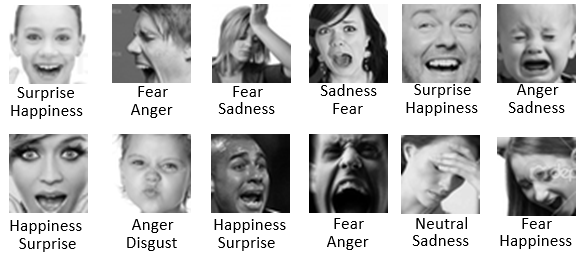
\includegraphics[width=10cm]{resources/fervsferplus.png}
  \caption{Comparison of FER and FERplus labels. Image obtained from the FERPlus paper\cite{BarsoumICMI2016}.}\label{fig:fervsferplus}
\end{figure}


\subsection{COCO 2014 dataset}

Microsoft released their COCO 2014 training dataset as part of a more extensive publication containing training, validation, and test images. Totaling 328K images, it was the largest and most curated dataset at its publication. The dataset contains 80 different classes and multiple captions per image. 


\subsection{Target styles for style transfer}


\begin{figure}[h]
  \centering
  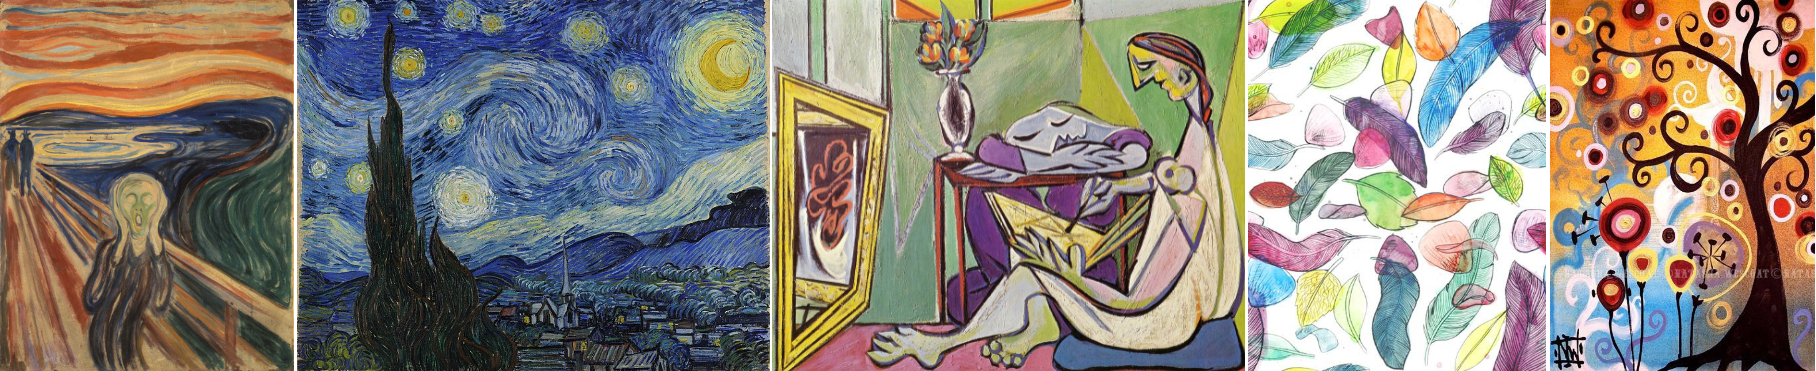
\includegraphics[width = 0.9\textwidth]{resources/target_styles.png}
  \caption{Target Styles. The corresponding assigned emotions, from left to right: Anger, Sadness, Fear, Happiness, Surprise.}
  \label{fig:target_styles}
\end{figure}

We selected five different paintings to be our target styles an assign them an emotion:
         \begin{itemize}
          \item \emph{The Scream} By Edvard Munch\footnote{From: https://www.edvardmunch.org/the-scream.jsp}  for the "anger" emotion, 
          \item \emph{The Starry Night} By Vincent Van Gogh\footnote{From: https://www.vangoghgallery.com/painting/starry-night.html} for the "Sadness" emotion,
          \item \emph{La Musa (Mujer Leyendo)} By Pablo Picasso\footnote{From: https://www.slobidka.com/pablo-picasso/158-picasso-la-musa-mujer-leyendo.html} for the "Fear" emotion,
          \item \emph{Feathers} By Kathryn Corlett\footnote{from: https://www.ebsqart.com/Artist/Natasha-Wescoat/1439/Art-Portfolio/June-Tree/717313/} for the "Hapiness" emotion,
          \item \emph{June tree} By Natasha Wescoat\footnote{From: http://kathryncorlett.blogspot.com/2012/05/wallpaper-feathers-petals-leaves.html} for the "Surprise" emotion.
\end{itemize}

These particular paintings were selected for various reasons. The first, is that some of them are widely used in other style transfer works, so we could compare qualitative results while we were developing them, like \emph{The scream} or \emph{The Starry Night}. We also found some target styles interesting enough to include them, like \emph{Feathers} and \emph{June tree}. 

The emotions assigned to each style were not pre-selected, meaning we did not select a particular style to portray a particular emotion, as the final style transfer image would sometimes not correspond to our pre-selected style. With \emph{The scream}, for instance, logic would have it that it would be selected to represent surprise or fear as that seems to be the motif of the painting, but in our results, we think the black and red hues and aggressive brushstrokes of the style-transferred image confer a more angry emotion rather than the other two.



\subsection{Methodology}
To achieve an MVP (Minimum Viable Product) and be worthy of an MSc project, we set our goals as the following:

\begin{itemize}
  \item Remove the need to use Google's Cloud API for all computer vision tasks, implementing local solutions.
  \item Implement new routines involving engaging computer vision algorithms like Style Transfer.
  \item The user should easily be able to obtain the style transferred files.
  \item The visual representation on the screen should be visually pleasing enough that users will want to keep it on as a background element.
  \item Make the robot completely autonomous: remove the need to offload computation to a 3rd party service or a local machine.
  \item Achieve a real-time representation of the robot's image processing.
\end{itemize}


\subsection{Face detection}

Previously, our pipeline for the robot required sending images to Google's Cloud Services (GCS) for emotion recognition. As we have removed GCS, this is no longer the case. To replace the previous face detection and emotion detection parts of the pipeline, we need to implement local face detection and emotion detection methods based on the current state of the art. Face detection allows the arm to follow a subject should it approach the camera's viewing angle limits. We propose using a Haar-Cascade classifier to detect faces. 

\subsection{Emotion recognition}
Detecting faces in the frame also serves to improve emotion detection. As described in Gunwan et al.\cite{haarcrop}, a neural network trained on cropped faces performs optimally on similarly cropped images. We propose training a network on the FERPlus\cite{BarsoumICMI2016} dataset.


\subsection{Style transfer method proposal}

We will use emotion recognition to change the context of the style transfer network, loosely adapting the target style transfer to a user's visible emotional status.


We propose a local implementation of a neural network capable of producing style transfer images as close to real-time on the Raspberry Pi 4's hardware as possible. The models can be pre-trained in a more powerful environment, but inference should run entirely locally on the device. This way, the robot does not need any external connections or dependencies in run-time. We propose experimenting with two different architectures: a recent model that requires more potent hardware but has better performance (results) and an older model that does not require high-end hardware, producing worse results but potentially giving us faster results and allowing the robot to run inference locally. Thus, we propose adapting Karras' StyleGAN2 representing the "state of the art" method, and since we are already using VGG16 and VGG19 models for our emotion recognition, adapting the method proposed by Justin Johnson et al. on their \emph{"Perceptual Losses for Real-Time Style Transfer
and Super-Resolution"} \cite{Johnson2016Perceptual} publication representing the "old but fast" method to run on our hardware.
While StyleGAN2 was trained using the FFHQ dataset \cite{nvlabs_2019}, we propose using Microsoft's COCO 2014 training dataset\cite{DBLP:journals/corr/LinMBHPRDZ14} to train our style transfer models, as we are not using only face images on our style transfer. 

If one of these two methods can run locally while achieving a good framerate, it should be strongly considered for the final implementation, as it would complete our final two objectives for an MVP.

\subsection{Combining everything to form a product}


We also need a way to get our style transferred images from the robot to the user. We propose using the Telegram Python API, implementing a Telegram bot that users can enable to receive their images on their mobile devices.

When we have all of our methods implemented, we will need a way to create a cohesive user experience through our robot. We need to design and implement a state machine that should conform to the following process:


\begin{enumerate}
  \item User powers the robot on.
  \item Robot searches for faces.
  \item When a face is found, recognize emotion and perform live style transfer.
  \item Whenever the user requests it, provide them with the style-transferred image file.
  \item Whenever the face is lost, go back to state 2)
\end{enumerate}